\documentclass{article}

\usepackage{arxiv}

\usepackage[utf8]{inputenc}
\usepackage[T1]{fontenc}
\usepackage{natbib}
\usepackage[french]{babel}
\usepackage{hyperref}
\usepackage{url}
\usepackage{booktabs}
\usepackage{multirow}
\usepackage{amsfonts}
\usepackage{amsmath}
\usepackage{nicefrac}
\usepackage{microtype}
\usepackage{graphicx}
\usepackage{subcaption}
\usepackage{float}
\usepackage{wrapfig}
\setlength{\textfloatsep}{6pt plus 2pt minus 2pt}
\setlength{\floatsep}{6pt plus 2pt minus 2pt}
\setlength{\intextsep}{6pt plus 2pt minus 2pt}
\setlength{\abovecaptionskip}{4pt}
\setlength{\belowcaptionskip}{2pt}
\raggedbottom
\usepackage{doi}

\title{Rapport Final --- Apprentissage par renforcement sur \textit{FrozenLake}}

\newif\ifuniqueAffiliation
\uniqueAffiliationtrue

\ifuniqueAffiliation
\author{
  Ibrahim R. HADJ-ARAB \\
  Faculté des sciences et de génie\\
  Université Laval\\
  \texttt{ibrahim-rabah.hadj-arab.1@ulaval.ca} \\
  \And
  Khalil EN NOUAARY \\
  Faculté des sciences et de génie\\
  Université Laval\\
  \texttt{khalil.en-nouaary.1@ulaval.ca} \\
}
\fi

\renewcommand{\shorttitle}{Rapport Final --- IFT-7201}

\hypersetup{
  pdftitle={Rapport final RL sur FrozenLake},
  pdfauthor={Ibrahim R. Hadj-Arab, Khalil En Nouaary},
}

\begin{document}
\maketitle

\noindent Code source disponible à : \url{https://github.com/Ribraba/IFT-7201-Projet}

\section{Cas d'étude}

\subsection{Composantes de l'environnement}

\textit{FrozenLake-v1}~\citep{towers2024} est un environnement de navigation en grille $N \times N$. L'espace d'états est l'ensemble des $N^2$ cases, représenté par un entier $s \in \{0, \ldots, N^2-1\}$ (numérotation de gauche à droite et de haut en bas) ; l'espace d'actions contient quatre déplacements (haut, bas, gauche, droite). Trois composantes peuvent être manipulées pour moduler la difficulté :

\begin{itemize}
  \item \textbf{Degré de stochasticité :} le paramètre \texttt{is\_slippery} contrôle la dynamique de transition. Lorsque activé, chaque action entraîne le déplacement souhaité avec probabilité $\nicefrac{1}{3}$ et l'un des deux déplacements perpendiculaires avec probabilité $\nicefrac{1}{3}$ chacun.
  \item \textbf{Nombre de situations dangereuses :} les cases de type \texttt{H} (trous) constituent les situations dangereuses. Augmenter leur nombre réduit la surface praticable et multiplie les risques de chute.
  \item \textbf{Positionnement des situations dangereuses :} regrouper les trous de façon contiguë crée un obstacle de type falaise, forçant l'agent à choisir entre un chemin court risqué et un détour sûr.
\end{itemize}

Un épisode se termine lorsque l'agent atteint l'objectif \texttt{G}, tombe dans un trou \texttt{H}, ou dépasse 200 pas de temps. La fonction de récompense est mise en forme (\textit{reward shaping}) pour accélérer la propagation du signal de danger sans modifier la politique optimale~\citep{ng1999} : chute ($r = -1{,}0$), objectif ($r = +1{,}0$), collision avec un mur ($r = -0{,}1$), déplacement ordinaire ($r = 0{,}0$).

\subsection{Cas d'étude}

\begin{figure}[h]
  \centering
  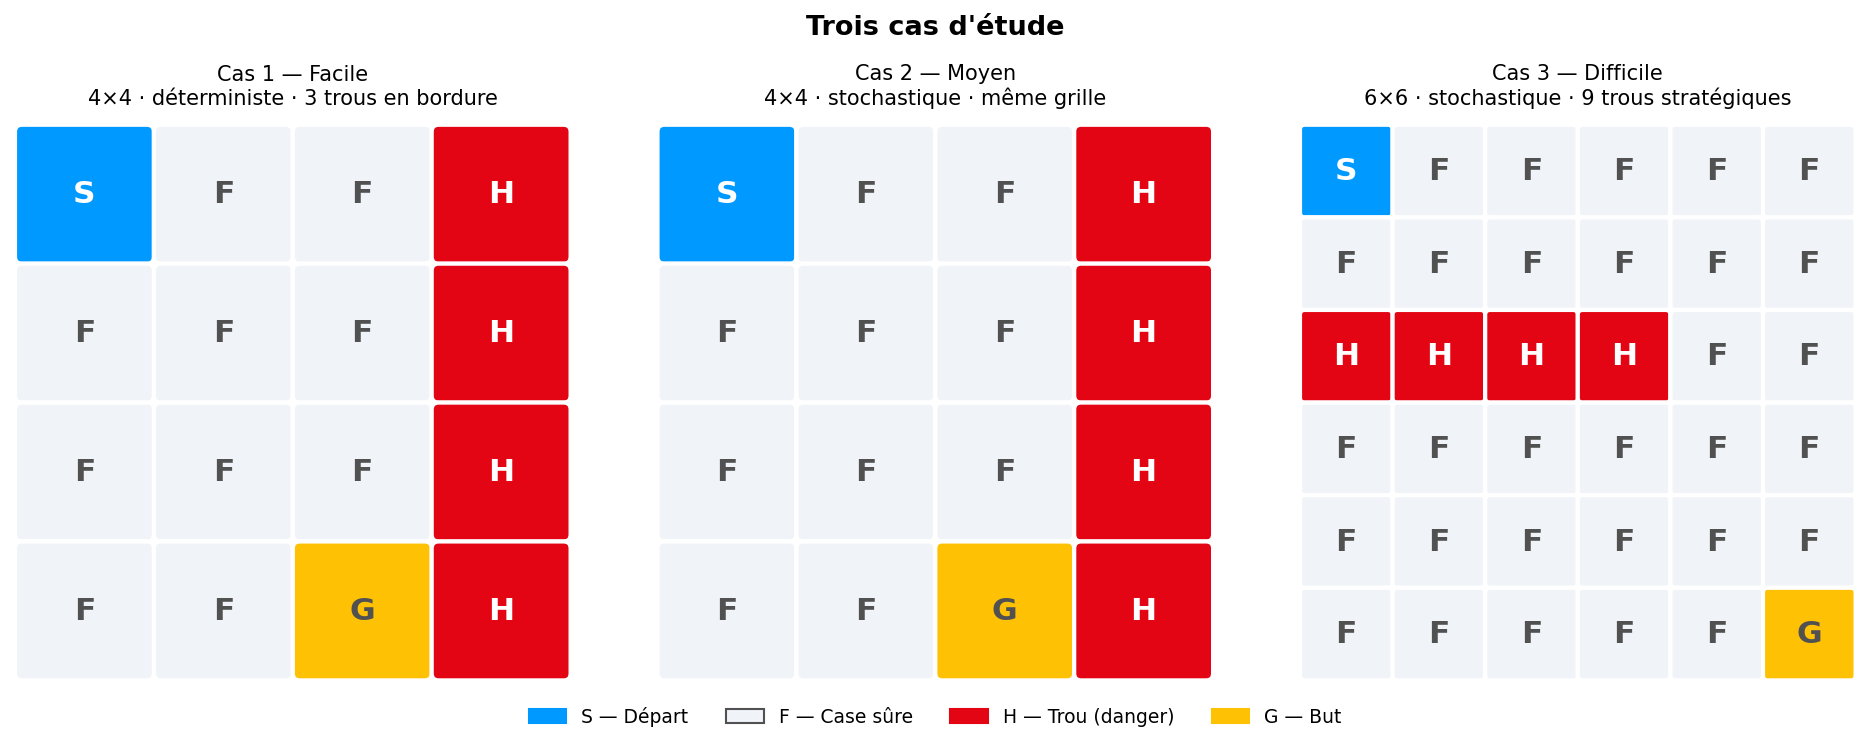
\includegraphics[width=0.72\linewidth]{../../figures/maps.png}
  \caption{Visualisation des trois environnements. \texttt{S} : départ, \texttt{G} : objectif, \texttt{H} : trou, \texttt{F} : case libre.}
  \label{fig:maps}
\end{figure}

Le Tableau~\ref{tab:configs} et la Figure~\ref{fig:maps} présentent les trois configurations retenues.

\begin{table}[h]
  \centering
  \caption{Configurations des trois cas d'étude.}
  \label{tab:configs}
  \small
  \begin{tabular}{lccc}
    \toprule
    & \textbf{Facile} & \textbf{Moyen} & \textbf{Difficile} \\
    \midrule
    Taille de la grille          & $4\times4$ & $4\times4$ & $6\times6$ \\
    \texttt{is\_slippery}        & Non & Oui & Oui \\
    Nombre de trous              & 3   & 3   & 4 \\
    Positionnement               & Colonne droite & Colonne droite & Rangée centrale \\
    \bottomrule
  \end{tabular}
\end{table}

\textbf{Facile} ($4\times4$, déterministe, 3 trous en colonne). Référence sans bruit : toute stratégie TD doit converger vers un taux de chutes nul. Valide l'implémentation et établit une borne supérieure de performance.

\textbf{Moyen} ($4\times4$, stochastique, 3 trous en colonne). Topologie identique à \textit{Facile} ; seul \texttt{is\_slippery} change. Isole proprement l'effet de la stochasticité sur la sécurité.

\textbf{Difficile} ($6\times6$, stochastique, 4 trous contigus en rangée centrale). La rangée \texttt{HHHHFF} crée une barrière horizontale analogue au \textit{cliff walking}~\citep[chap.~6]{sutton2018}. Deux trajectoires coexistent : un chemin court risqué longeant les trous et un long détour sûr par les colonnes droites. La grille $6\times6$ assure que ce détour est significativement plus long, condition nécessaire pour observer la divergence \textit{off-policy}/\textit{on-policy}.


\section{Stratégies considérées}

Deux stratégies de différence temporelle (TD) sont sélectionnées comme baselines : Q-learning et SARSA. Ces méthodes ne disposent d'aucun mécanisme conçu explicitement pour éviter les situations dangereuses, établissant ainsi une limite de référence. Le choix de méthodes tabulaires (plutôt que DQN~\citep{mnih2015} ou PPO) se justifie par la taille réduite de l'espace d'états ($16$ et $36$ états) : les différences observées reflètent directement les propriétés intrinsèques des algorithmes. Q-learning et SARSA forment la paire canonique \textit{off-policy}/\textit{on-policy} dont les comportements face aux obstacles sont directement prédits par la théorie~\citep{sutton2018}.

\textbf{Q-learning}~\citep{watkins1992} est une méthode \textit{off-policy} dont la règle de mise à jour est :
\begin{equation}
  Q(s, a) \leftarrow Q(s, a) + \alpha \bigl[r + \gamma \max_{a'} Q(s', a') - Q(s, a)\bigr].
\end{equation}
En ciblant toujours le maximum, Q-learning peut sous-estimer le risque réel et préférer le chemin court risqué dans des environnements à obstacles groupés.

\textbf{SARSA}~\citep{rummery1994} est une méthode \textit{on-policy} qui utilise l'action réellement sélectionnée :
\begin{equation}
  Q(s, a) \leftarrow Q(s, a) + \alpha \bigl[r + \gamma\, Q(s', a') - Q(s, a)\bigr].
\end{equation}
Puisque $a'$ peut être aléatoire (avec probabilité $\varepsilon$), SARSA intègre le coût de l'exploration dans ses estimations, ce qui le rend naturellement plus prudent près des obstacles.

Trois travaux en Safe Reinforcement Learning ont été identifiés, chacun proposant un mécanisme distinct d'intégration de la sécurité.

\textbf{Model-based Safe Deep RL via a Constrained Proximal Policy Optimization Algorithm}~\citep{CMDP2022} étend PPO en couplant un modèle de dynamique appris avec une optimisation sous contraintes de coût cumulé (CMDP). L'agent anticipe les conséquences futures avant d'agir, offrant des garanties théoriques solides, mais cette méthode repose fondamentalement sur l'approximation de fonction et l'apprentissage profond, la rendant peu adaptée à un cadre tabulaire.

\textbf{Safe RL by Imagining the Near Future}~\citep{Future2022} adopte une stratégie prédictive : l'agent apprend un modèle du monde et simule des trajectoires futures avant d'agir pour évaluer le risque à court terme. Cette anticipation évite certaines erreurs a priori, mais le modèle neuronal et la génération de trajectoires imaginées sont difficilement transposables à un cadre où les transitions sont déjà exactement connues.

\textbf{The Fear Field Framework}~\citep{Fearfield2025} propose un shielding adaptatif pour environnements stochastiques discrets. La méthode maintient dynamiquement une zone tampon autour des états dangereux, appelée \textit{fear field}, dont le rayon s'élargit lors de transitions imprévues et se réduit en l'absence d'incident. Un mécanisme d'exploration adaptative augmente $\varepsilon$ lorsqu'un comportement de boucle est détecté.

Parmi ces trois approches, le \textbf{principe du shielding adaptatif} proposé par Fear Field est retenu comme stratégie principale. C'est l'approche la plus récente (2025), directement appliquée à \texttt{FrozenLake-v1} par ses auteurs~\citep{Fearfield2025}, et la seule adaptable à un cadre tabulaire sans réseau de neurones. Son mécanisme répond précisément au défi central de l'étude : la stochasticité de \texttt{is\_slippery=True}, où les glissades imprévues rendent les politiques naïves vulnérables.

Notre adaptation tabulaire remplace le modèle neuronal original par la table de transitions exacte de Gymnasium (\texttt{env.unwrapped.P}), éliminant tout apprentissage auxiliaire tout en préservant l'idée centrale du shielding prédictif. Nous ne conservons pas le mécanisme d'exploration adaptative ni le rétrécissement progressif du rayon, ces aspects introduisant des hyperparamètres supplémentaires hors du cadre de cette étude.

Avant chaque sélection d'action, l'ensemble des actions admissibles est déterminé :
\begin{equation}
  \mathcal{A}_{\text{safe}}(s) = \left\{ a \in \mathcal{A} \;\middle|\;
  \forall\, (p,\, s',\, r,\, d) \in P(s,\, a),\quad p > 0
  \Rightarrow s' \notin \mathcal{H} \right\}
\end{equation}
où $\mathcal{H}$ est l'ensemble des états-trous. Si $\mathcal{A}_{\text{safe}}(s) = \emptyset$, toutes les actions sont autorisées (cas de repli). La sélection $\varepsilon$-greedy est restreinte à cet ensemble :
\begin{equation}
  a_t = \begin{cases}
    \text{Uniform}\!\left(\mathcal{A}_{\text{safe}}(s_t)\right) & \text{avec probabilité } \varepsilon \\[4pt]
    \displaystyle\arg\max_{a\,\in\,\mathcal{A}_{\text{safe}}(s_t)} Q(s_t,\, a) & \text{sinon}
  \end{cases}
\end{equation}
La mise à jour TD demeure identique à Q-learning standard. La différence fondamentale est que l'exploration et l'exploitation sont toutes deux contraintes à $\mathcal{A}_{\text{safe}}(s)$, empêchant toute sélection d'une action menant vers un trou pendant l'apprentissage.


\section{Méthodologie expérimentale}

\textbf{Librairies :} l'environnement est fourni par Gymnasium~1.2.3~\citep{towers2024}. Les trois algorithmes sont implémentés en Python/NumPy~2.2.6, sans recours à Stable-Baselines3~\citep{raffin2021}, afin de contrôler précisément les mises à jour TD et la construction du shield.

\textbf{Hyper-paramètres :} les trois algorithmes partagent les mêmes hyper-paramètres : $\gamma = 0{,}99$, $\alpha_0 = 0{,}5$~\citep{sutton2018}, décroissance $0{,}9995$ pour $\alpha$ et $\varepsilon$ jusqu'aux minima $\alpha_{\min}=0{,}01$ et $\varepsilon_{\min}=0{,}05$ (atteints après $\approx\!6\,000$ épisodes). Le Q-learning blindé n'introduit aucun hyper-paramètre supplémentaire : le shield est construit directement depuis \texttt{env.unwrapped.P}.

\textbf{Paramètres expérimentaux :} chaque configuration est entraînée sur 20\,000 épisodes (maximum 200 pas). Les expériences sont répétées avec $n=10$ graines indépendantes. L'évaluation finale utilise la politique greedy ($\varepsilon=0$, sans shield) sur 500 épisodes.

\textbf{Indicateurs de performance :}
\begin{itemize}
  \item \textbf{Récompense et taux de chutes durant l'entraînement} (moyenne mobile, fenêtre 500~épisodes) : convergence et sécurité au cours de l'apprentissage.
  \item \textbf{Taux de boucles durant l'entraînement} : fraction d'épisodes terminés par dépassement de la limite de pas.
  \item \textbf{Taux d'états dangereux à l'évaluation} : fraction de pas dans une case adjacente à un trou lors de la politique greedy.
  \item \textbf{Taux de chemins sécurisés à l'évaluation} : fraction des épisodes réussis dont la trajectoire chevauche à $\geq 50\,\%$ le chemin optimal de sécurité calculé par Dijkstra~\citep{dijkstra1959} (cas Difficile uniquement).
\end{itemize}

\section{Résultats}

\begin{figure}[H]
  \centering
  \begin{subfigure}[t]{0.32\linewidth}
    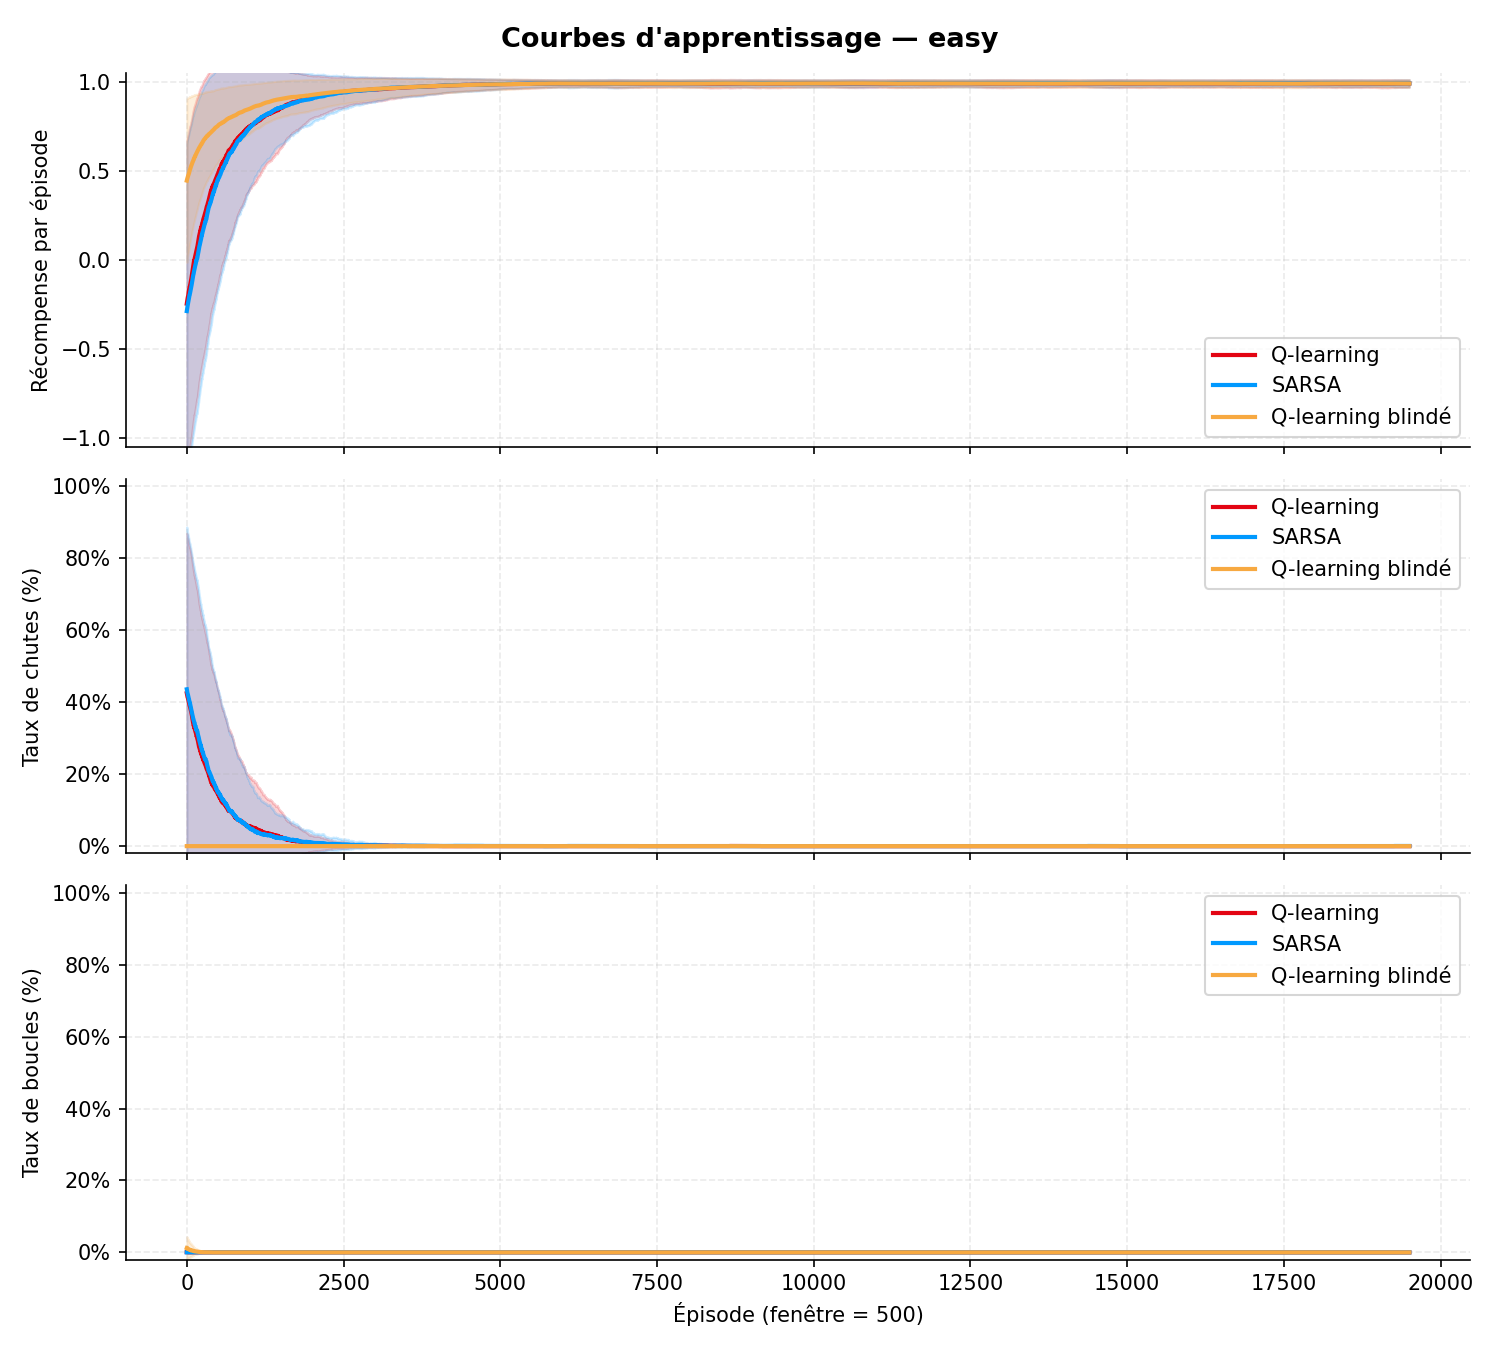
\includegraphics[width=\linewidth]{../../figures/training_easy.png}
    \caption{\textbf{Facile} : convergence rapide vers 0\,\% de chutes. Le shield n'apporte aucun avantage dans l'environnement déterministe.}
  \end{subfigure}
  \hfill
  \begin{subfigure}[t]{0.32\linewidth}
    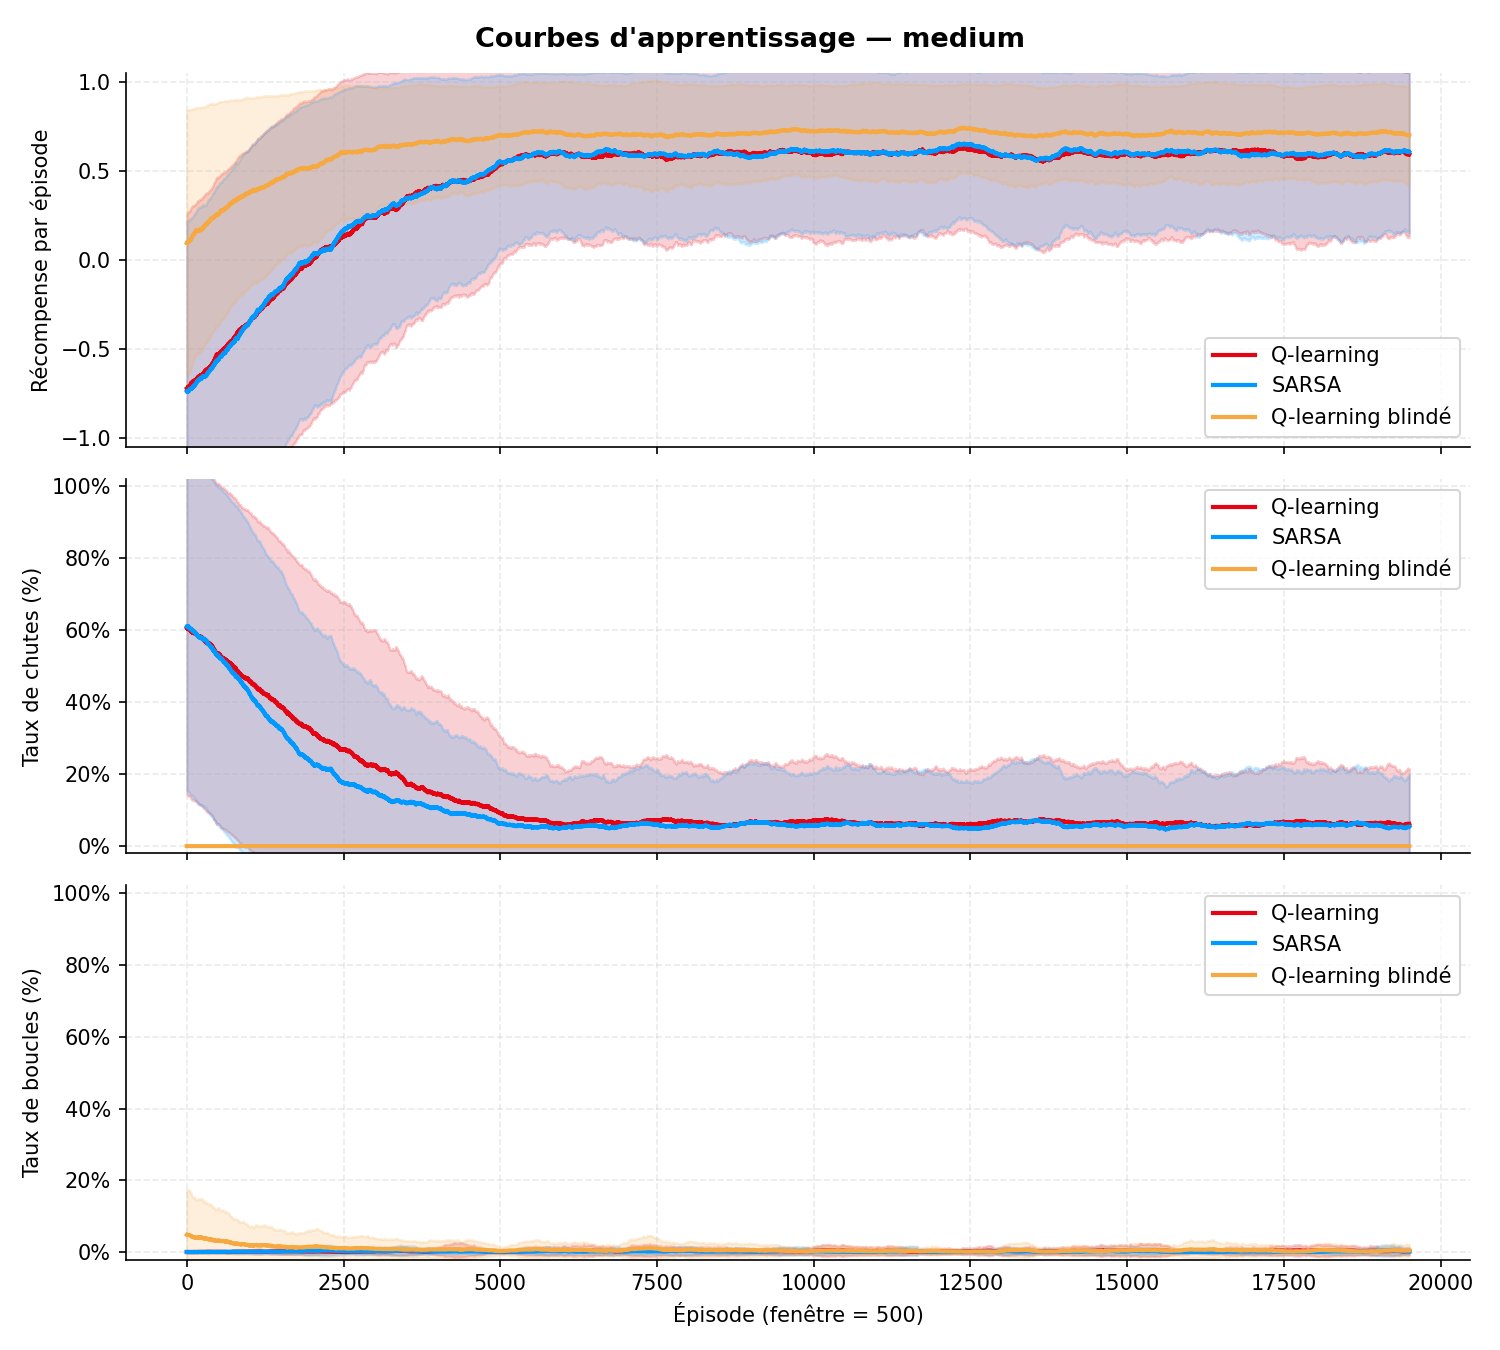
\includegraphics[width=\linewidth]{../../figures/training_medium.png}
    \caption{\textbf{Moyen} : la stochasticité maintient un risque résiduel. Le shield réduit les chutes en début d'apprentissage par rapport aux baselines.}
  \end{subfigure}
  \hfill
  \begin{subfigure}[t]{0.32\linewidth}
    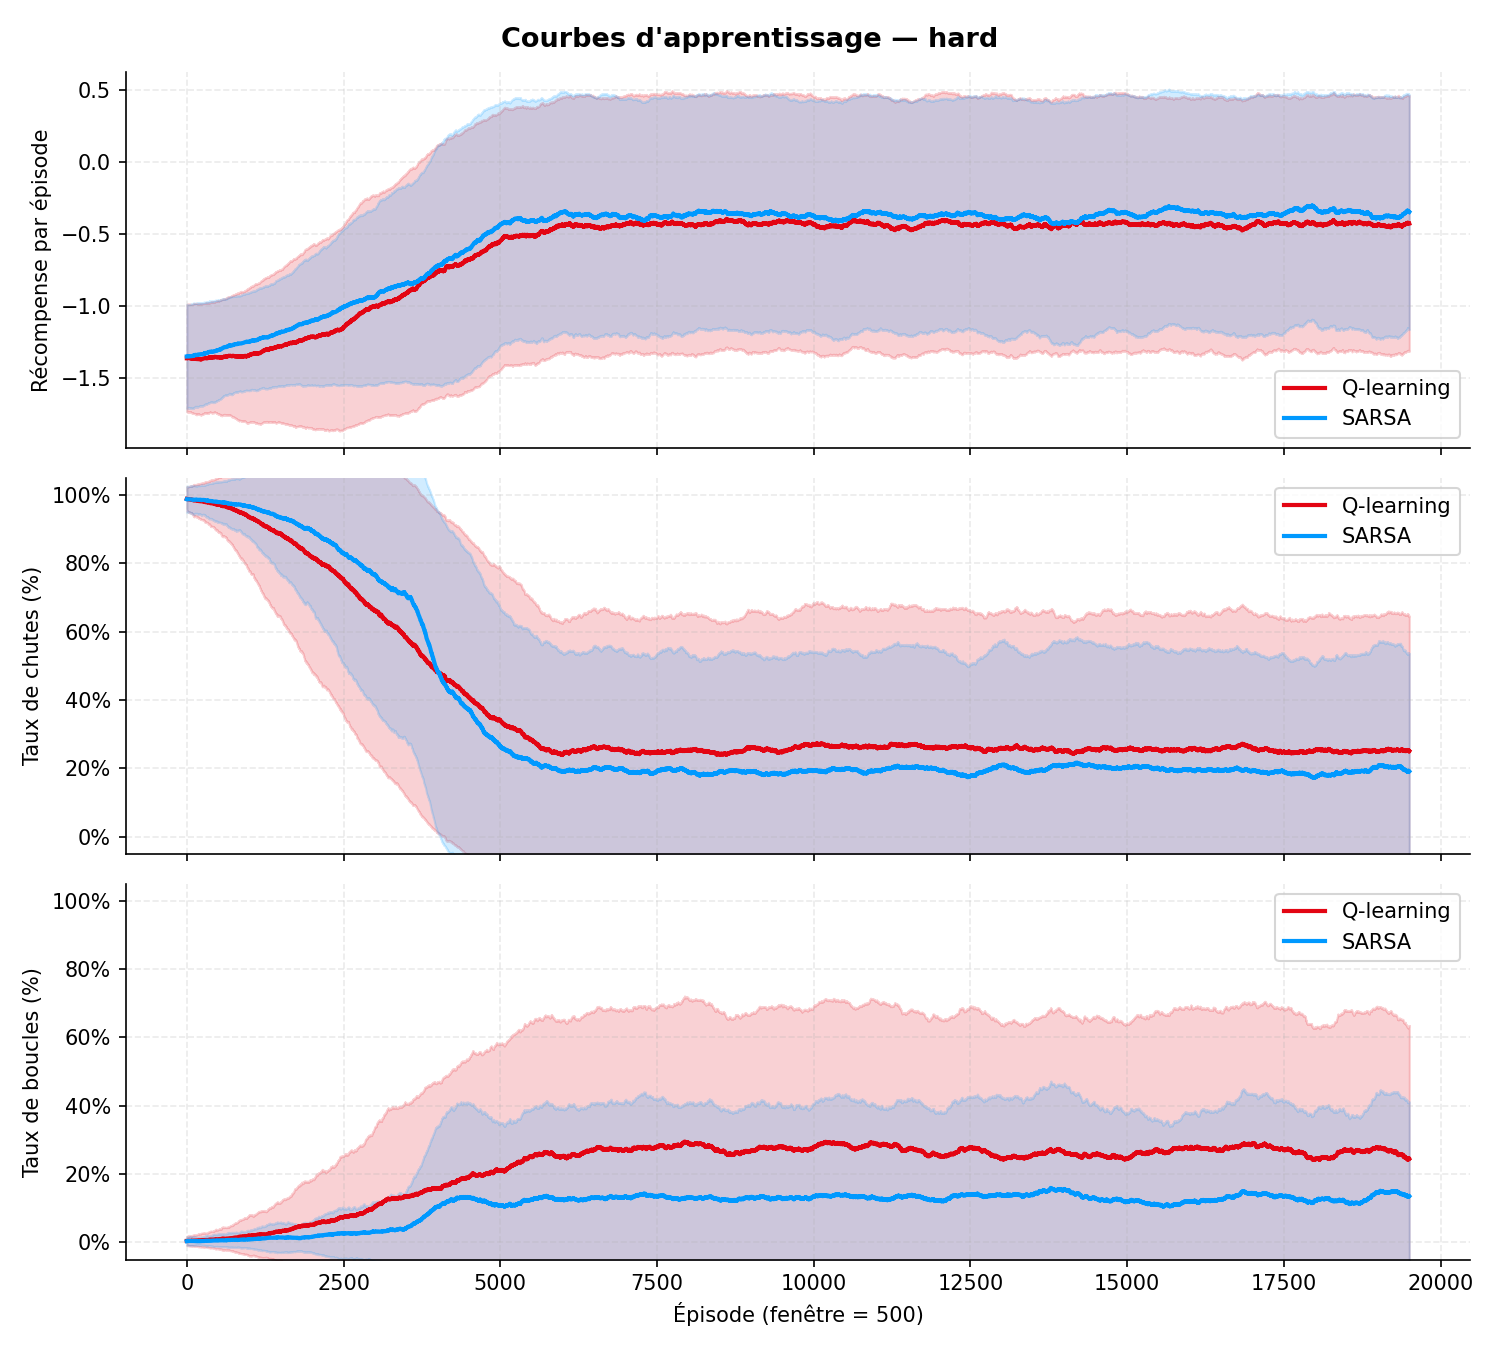
\includegraphics[width=\linewidth]{../../figures/training_hard.png}
    \caption{\textbf{Difficile} : SARSA et le shield réduisent davantage les chutes que Q-learning en fin d'apprentissage.}
  \end{subfigure}
  \caption{Courbes d'apprentissage (récompense, chutes, boucles). Bande colorée : $\pm$ un écart-type sur 10 répétitions. \textit{Facile} valide l'implémentation ; \textit{Moyen} isole la stochasticité ; \textit{Difficile} révèle la divergence \textit{off-policy}/\textit{on-policy}.}
  \label{fig:train_all}
\end{figure}

\begin{figure}[H]
  \centering
  \begin{subfigure}[t]{0.49\linewidth}
    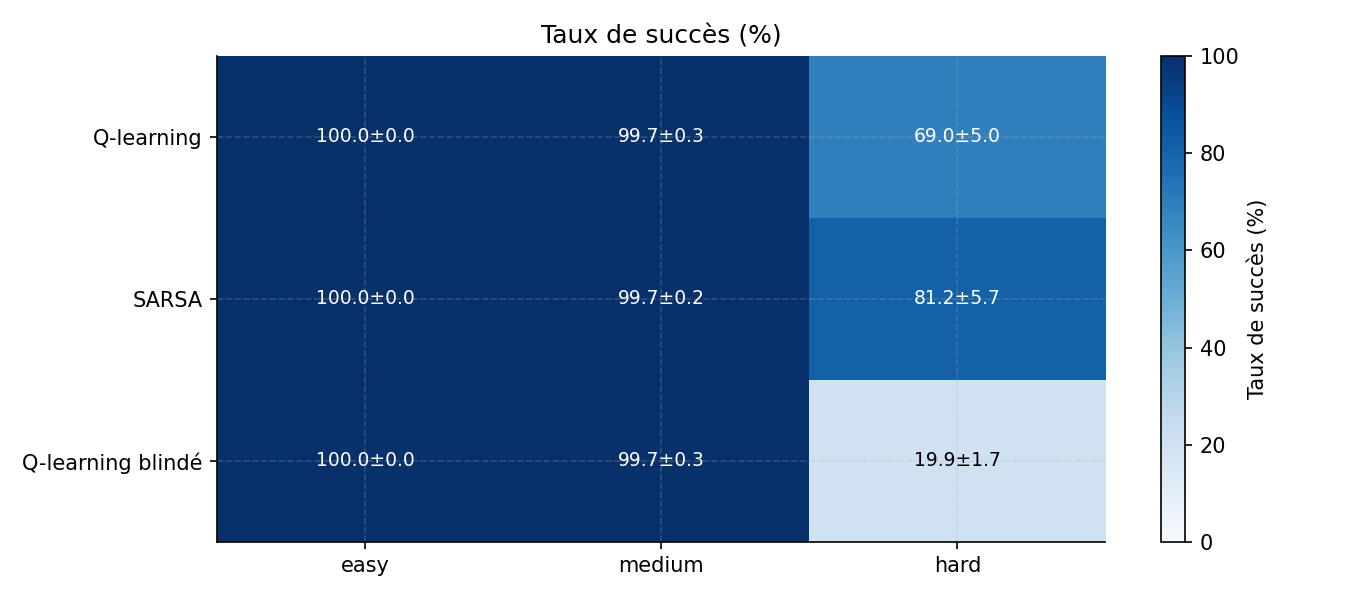
\includegraphics[width=\linewidth]{../../figures/overview_success_rate.png}
    \caption{Taux de succès à l'évaluation.}
  \end{subfigure}
  \hfill
  \begin{subfigure}[t]{0.49\linewidth}
    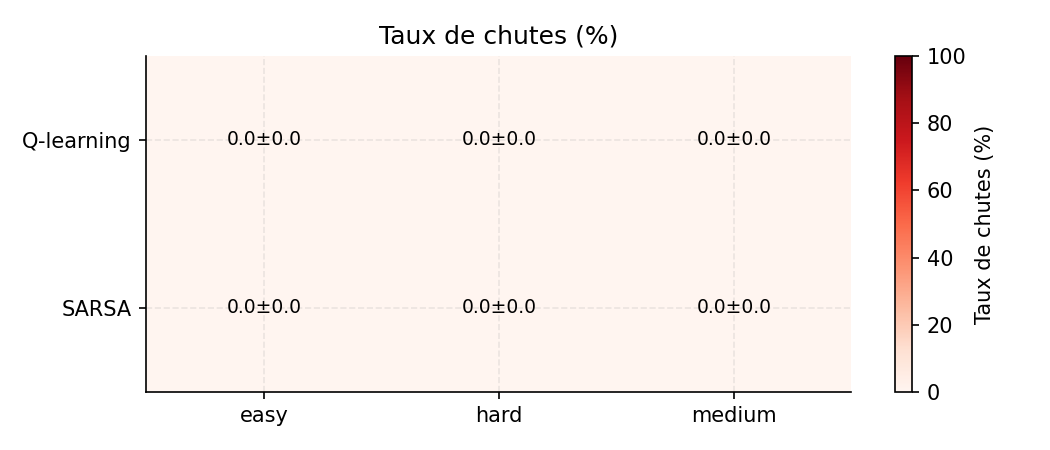
\includegraphics[width=\linewidth]{../../figures/overview_fall_rate.png}
    \caption{Taux de chutes à l'évaluation.}
  \end{subfigure}
  \caption{Vue d'ensemble : évaluation greedy sans shield, 500 épisodes. Le taux de chutes élevé du Q-learning blindé sur \textit{Difficile} est absent sur les deux autres cas.}
  \label{fig:overview}
\end{figure}

\begin{table}[H]
  \centering
  \begin{minipage}[c]{0.62\linewidth}
    \caption{Indicateurs d'évaluation finale (politique greedy sans shield, 500 épisodes, moyenne $\pm$ écart-type, 10 répétitions). Chemin sûr : chevauchement $\geq 50\%$ avec Dijkstra (Difficile uniquement).}
    \label{tab:eval}
    \scriptsize
    \begin{tabular}{llccc}
      \toprule
      & & \textbf{Facile} & \textbf{Moyen} & \textbf{Difficile} \\
      \midrule
      \multirow{5}{*}{Q-learning}
        & Succès      & $100{,}0 \pm 0{,}0\%$ & $99{,}7 \pm 0{,}3\%$ & $69{,}0 \pm 5{,}0\%$ \\
        & Chutes      & $0{,}0 \pm 0{,}0\%$   & $0{,}0 \pm 0{,}0\%$  & $0{,}0 \pm 0{,}0\%$ \\
        & Boucles     & $0{,}0 \pm 0{,}0\%$   & $0{,}3 \pm 0{,}3\%$  & $31{,}0 \pm 5{,}0\%$ \\
        & Danger      & $20{,}0\%$             & $28{,}5\%$           & $29{,}9\%$ \\
        & Chemin sûr  & {-}{-}{-}             & {-}{-}{-}            & $60{,}1 \pm 2{,}9\%$ \\
      \midrule
      \multirow{5}{*}{SARSA}
        & Succès      & $100{,}0 \pm 0{,}0\%$ & $99{,}7 \pm 0{,}2\%$ & $81{,}2 \pm 5{,}7\%$ \\
        & Chutes      & $0{,}0 \pm 0{,}0\%$   & $0{,}0 \pm 0{,}0\%$  & $0{,}0 \pm 0{,}0\%$ \\
        & Boucles     & $0{,}0 \pm 0{,}0\%$   & $0{,}3 \pm 0{,}2\%$  & $18{,}8 \pm 5{,}7\%$ \\
        & Danger      & $20{,}0\%$             & $27{,}7\%$           & $25{,}9\%$ \\
        & Chemin sûr  & {-}{-}{-}             & {-}{-}{-}            & $70{,}4 \pm 2{,}9\%$ \\
      \midrule
      \multirow{5}{*}{\shortstack{Q-l.\\blindé}}
        & Succès      & $100{,}0 \pm 0{,}0\%$ & $99{,}7 \pm 0{,}3\%$ & $19{,}9 \pm 1{,}7\%$ \\
        & Chutes      & $0{,}0 \pm 0{,}0\%$   & $0{,}0 \pm 0{,}0\%$  & $75{,}2 \pm 2{,}2\%$ \\
        & Boucles     & $0{,}0 \pm 0{,}0\%$   & $0{,}3 \pm 0{,}3\%$  & $4{,}9 \pm 1{,}4\%$ \\
        & Danger      & $20{,}0\%$             & $28{,}6\%$           & $30{,}4\%$ \\
        & Chemin sûr  & {-}{-}{-}             & {-}{-}{-}            & $68{,}7 \pm 2{,}6\%$ \\
      \bottomrule
    \end{tabular}
  \end{minipage}\hfill
  \begin{minipage}[c]{0.35\linewidth}
    \small
    Sur Facile et Moyen, les trois stratégies sont équivalentes à l'évaluation. Sur Difficile, le Q-learning blindé obtient seulement $19{,}9\%$ de succès avec $75{,}2\%$ de chutes, bien en dessous de SARSA ($81{,}2\%$) et de Q-learning ($69{,}0\%$). Son taux de boucles ($4{,}9\%$) est pourtant le plus faible ; c'est la politique greedy sans shield qui marche fréquemment vers les trous.
  \end{minipage}
\end{table}

\begin{figure}[H]
  \centering
  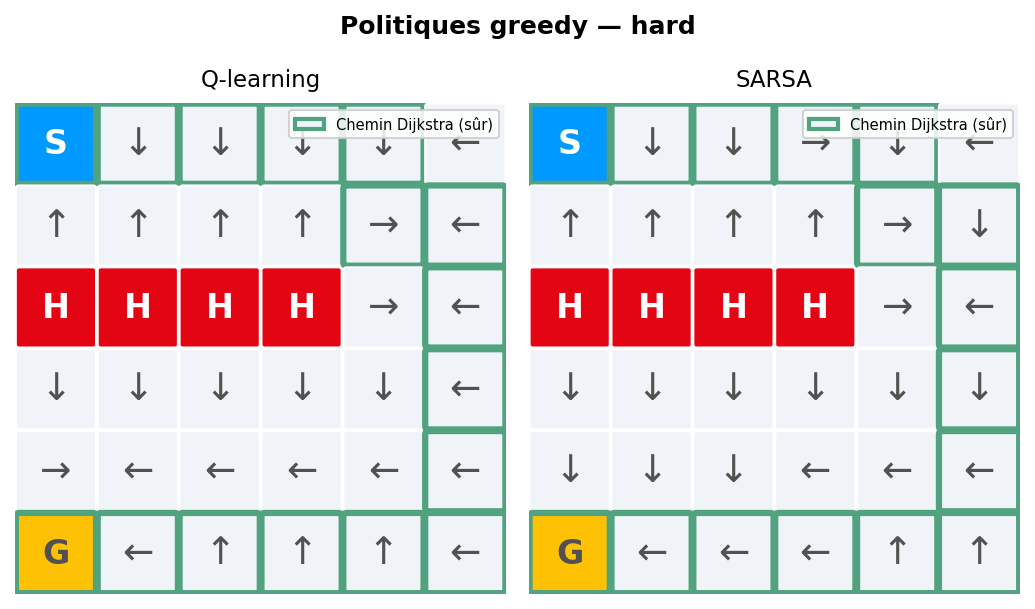
\includegraphics[width=\linewidth]{../../figures/policy_hard.png}
  \caption{Politiques greedy sur le cas Difficile (10 répétitions). Le contour vert délimite le chemin Dijkstra. SARSA emprunte systématiquement le détour sûr. Le Q-learning blindé présente des flèches incohérentes dans la zone proche de la barrière, signe d'une table Q mal calibrée sans shield actif.}
  \label{fig:policy_hard}
\end{figure}

\section{Discussion}

\textbf{Liens avec la littérature :} sur le cas Difficile, SARSA emprunte le détour sûr plus souvent que Q-learning ($70{,}4\%$ contre $60{,}1\%$), confirmant le phénomène du \textit{cliff walking} prédit par la théorie~\citep[chap.~6]{sutton2018} : la mise à jour \textit{on-policy} intègre naturellement le coût de l'exploration dans les estimations de valeur. La réduction des chutes par le shield pendant l'entraînement est cohérente avec le principe Fear Field~\citep{Fearfield2025}. Cependant, l'implémentation originale maintient le shield au déploiement, alors que notre évaluation greedy ne l'applique pas. Cette différence de protocole est à l'origine de la dégradation observée sur le cas Difficile.

\textbf{Explication des résultats :} sur Facile et Moyen, les trois stratégies convergent vers des politiques équivalentes. Sur Difficile, le problème vient de la contrainte $\mathcal{A}_{\text{safe}}(s)$ : les actions vers les trous n'étant jamais sélectionnées pendant l'entraînement, leurs Q-valeurs restent à leur valeur initiale nulle. À l'évaluation sans shield, ces valeurs nulles deviennent compétitives avec celles des chemins longs qui contournent la barrière, et l'agent tombe dans $75{,}2\%$ des cas. S'ajoute à cela que pour les états proches de la barrière centrale, $\mathcal{A}_{\text{safe}}(s) = \emptyset$ : le shield est désactivé par le repli précisément là où il devrait protéger l'agent, laissant les Q-valeurs de cette zone mal estimées. En résumé, sécuriser l'exploration peut dégrader la politique finale si le shield n'est pas actif au déploiement.

\textbf{Réflexion :} SARSA offre le meilleur rapport qualité-sécurité sans mécanisme dédié : sa mise à jour \textit{on-policy} produit la meilleure politique finale sur Difficile ($81{,}2\%$ de succès, $25{,}9\%$ de proximité aux trous). Le shield tabulaire est computationnellement léger ($O(|\mathcal{S}| \times |\mathcal{A}|)$ par épisode), mais sa principale limite pratique est la nécessité de connaître $P(s'|s,a)$ exactement. Dans un système réel, cette table devrait être apprise, ce qui introduit des erreurs de modèle. Deux extensions naturelles seraient d'appliquer le shield aussi à l'évaluation, ou de remplacer la contrainte stricte ($p > 0$) par un seuil probabiliste ($p > \theta$) pour réduire la sur-conservativité en environnement stochastique.

\textbf{Message général au client :} réduire les situations dangereuses pendant l'apprentissage est atteint par les trois stratégies — aucune chute n'apparaît à la politique finale sur Facile et Moyen. Sur l'environnement le plus difficile, le Q-learning blindé simplifié montre ses limites avec $75{,}2\%$ de chutes à l'évaluation greedy. La recommandation est d'utiliser \textbf{SARSA} comme base pour les environnements stochastiques à obstacles groupés, et de combiner cette approche avec un shield maintenu au déploiement si des garanties de sécurité formelles sont nécessaires à chaque pas de décision.

\newpage
\bibliographystyle{unsrtnat}
\bibliography{references}

\end{document}
